\chapter{Background}
General discription of used terms/systems in wikipedia like style. This means the description should not be too extensive.
And refer to further papers for more extensive descriptions.
\section{Wireless Networks}
  Wireless networks are computer networks which use radio-waves instead of cables in order two communicate.
  They are used in scenarios where using wires for connections are not possible or cumbersome like systems where devices are mobile.
  There are different scales where wireless connections are utilized:
    \begin{itemize}
      \item Smallish systems like a \ac{PAN} where a smartphone would use bluetooth to connect to headphones or glasses. Typical range for this field of
	application is within a few meters.
      \item Medium Sized systems like a \ac{WLAN} with laptops or smartphones connecting to an infrastructure through a wireless accesspoint.
	Typical range is about 50 meters.
      \item Large scale systems like television broadcasting with \ac{DVB-T} through satellites with typical ranges of up to 35400 kilometers.
    \end{itemize}
  \subsection{Wireless Access-Point}
    Is a device which allows other devices with wireless adapters to connect to its network.
    Mostly it serves as an entry point to a network-infrastructure and ultimately the internet like a common network switch, 
    but accesspoints have more modes of operation. Those are in general the following
    \begin{description}
      \item[Infrastructure-mode]
	Using this mode, the clients connect themselves to the accesspoints in order to get access to the network behind the accesspoints, like fileservers or the internet.
	To do so one or more accesspoints announce their services through small broadcasted packets called beacons, which include a \ac{SSID}, 
	the name/identifier of the wireless network. This is done 
	so that multiple wireless networks can be differentiated from each other. Those SSIDs, if received, are then used by the clients to
	establish a link to the herein before mentioned accesspoints.
      \item [Ad-hoc-mode]
	In an ad-hoc network all participants (accesspoints and clients) use the same \ac{SSID} and create spontaneous connections between each other in order to 
	exchange data. Note that also the former end-user-devices like laptops or smartphones are now nodes in this network and route packets instead of just originating or
	terminating them. \cite{Akyildiz2005445}.
     \item [Client-mode]
	Here the accesspoint acts the same as the wireless adapter of ordinary end-user-devices and establish links to other infrastructure-serving accesspoints or 
	ad-hoc systems. For example a laptop could be connected to an accesspoint through wire and then this accesspoint connects iteself to another network.
    \end{description}
    
  \subsection{\ac{WMN}}
    A mesh is a topology with no firm structure. Therefore a wireless mesh network is a network of wireless devices creating a mesh topology with connections between the participants.
    A Wireless mesh network consist of mesh routers and mesh clients, where routers form the backbone and forward packets on behalf of other nodes (especially the clients).
    Due to their autonomy and dynamic self-organization, the nodes in such a network create spontaneous ad-hoc networks in a locally optimal fashion.
    This trait provides the network with a greater resilience to node and connection failures (self-healing capabilities), 
    as spontaneously new connections are established between the nodes and redundand or backup paths are formed. 
    The drawback of this feature lies in its declining performance with increasing size of the network due to the locally optimal choices.
    The IEEE 802.11s standard describes how to from such wireless mesh networks. \cite{GRH_WLANMeshStandard_IEEEWiCom2010} 
    \begin{figure}[t]
      \centering
      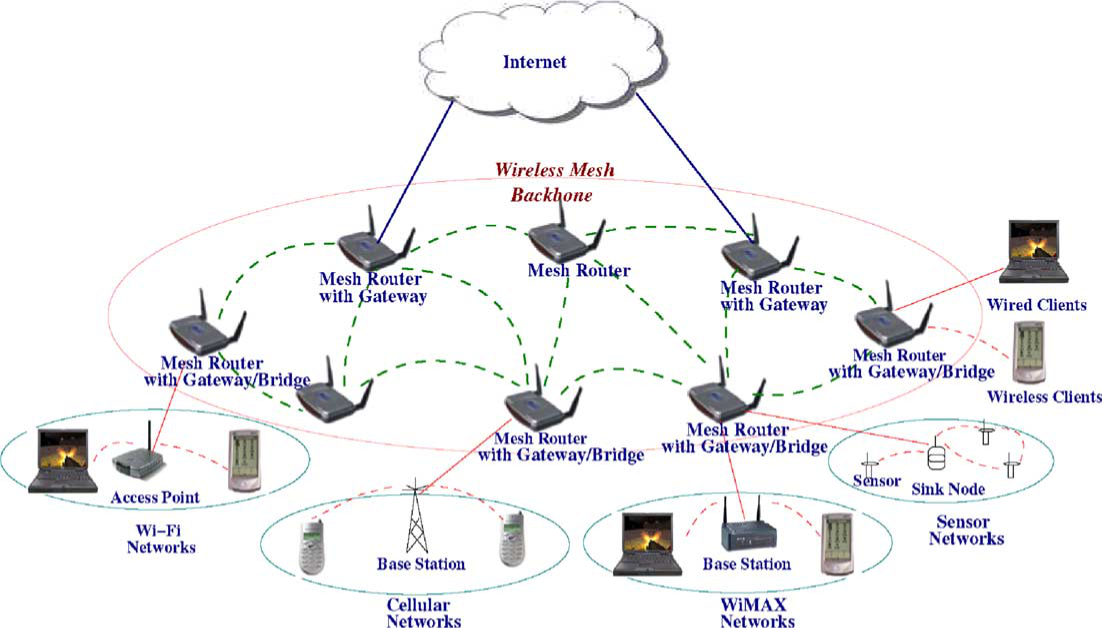
\includegraphics[width=0.8\columnwidth]{figures/mesh.png}
      \caption{A \ac{WMN} illustrated by \cite{Akyildiz2005445}}
      \label{fig:mesh}
    \end{figure}
    
  \subsection{\ac{WLAN} Channel}
    A \ac{WLAN} Channel as specified by IEEE 802.11 family uses a specific frequency-range in the \ac{UHF} or \ac{SHF} radio-scope in order to digitally modulate data on carrier waves.
    This is done to transmit data from a Sender station to a receiver station and creates a link between two Nodes in a \ac{WMN}. 
    
    \ac{WLAN} uses the two license-free frequency bands at 2.4Ghz and additionally certain bands at 5Ghz.
    \begin{figure}[t]
      \centering
      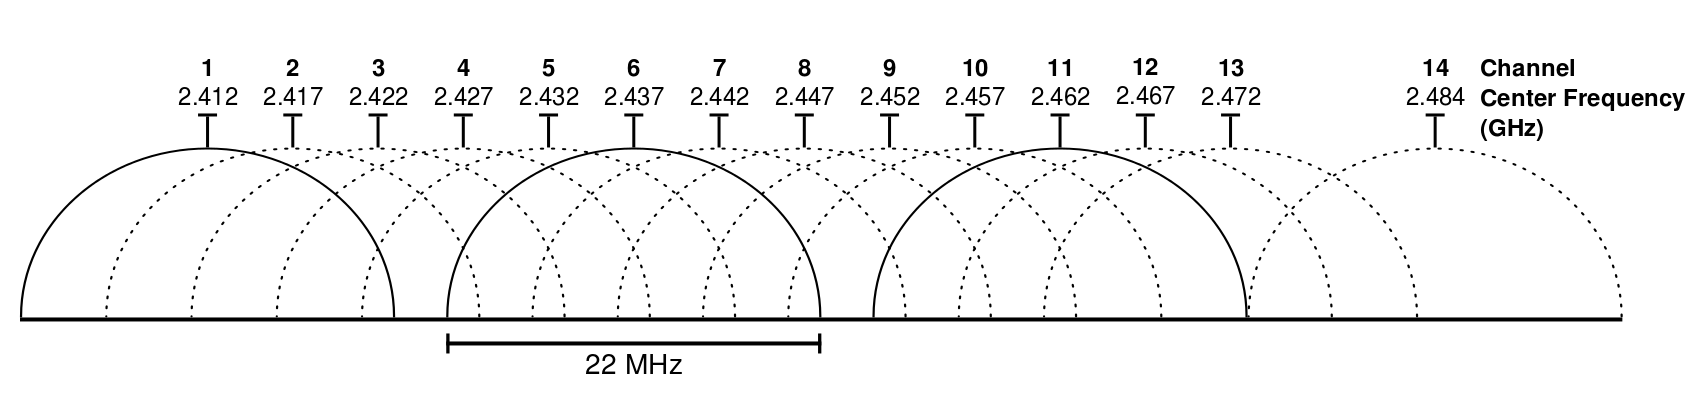
\includegraphics[width=0.8\columnwidth]{figures/wlan_channels.png}
      \caption{Mapping of channels to frequencies for the 2.4 Ghz band. \cite{wlan_channels}}
      \label{fig:wlan_channels}
    \end{figure}
    As we can see in \ref{fig:wlan_channels}, certain channels have overlapping regions.
    
      \subsubsection{\ac{CSMA/CA}}
	\ac{CSMA/CA} is a network protocol that describes how to access a shared medium, like a shared WLAN channel.
	It works as described by the following:
	\begin{quotation}
	  CSMA works on the principle that only one device can transmit signals on the network, 
	  otherwise a collision will occur resulting in the loss of data packets or frames. 
	  CSMA works when a device needs to initiate or transfer data over the network. 
	  Before transferring, each CSMA must check or listen to the network for any other transmissions that may be in progress. 
	  If it senses a transmission, the device will wait for it to end. Once the transmission is completed, 
	  the waiting device can transmit its data/signals. However, if multiple devices access it simultaneously and a collision occurs, 
	  they both have to wait for a specific time before reinitiating the transmission process. 
	\end{quotation} \cite{csma_techo}
	
	The Hidden-Station-Problem describes an undesired scenario where an Accesspoint B is in range of A and C but A and C are note in range, see \ref{fig:csmaca}.
	
	\begin{figure}[t]
	  \centering
	  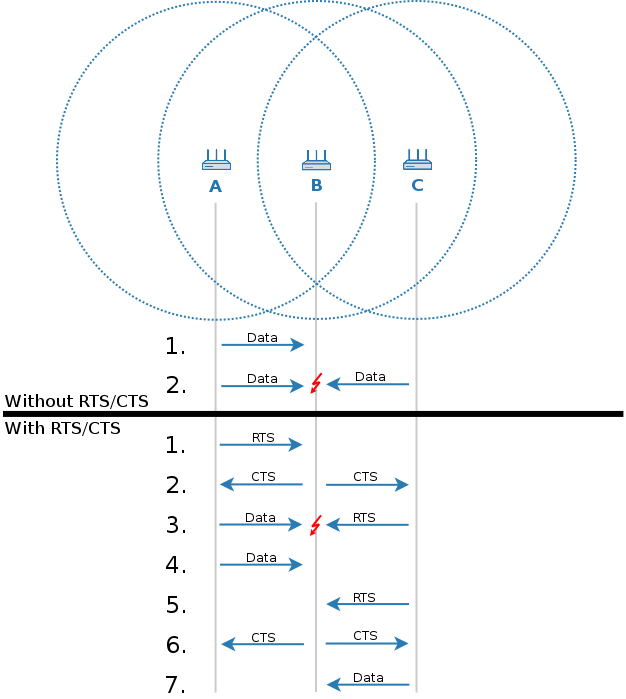
\includegraphics[width=0.8\columnwidth]{figures/csmaca.png}
	  \caption{Hidden-Station Problem and the RTS/CTS solution. When A sends data to B in Step 1, 
	    it first waits until the medium is free and then begins transmitting its data to B. 
	    Because of the range-limitation, C does not recognize the transmission of A to B. 
	    If B then wants to also transmit data to B, it also checks if the medium is free, which it falsely assumes
	    and then starts to transmit its data. This leads to collisions at B in step 2 and the data received will be corrupt.
	    The RTS/CTS protocol tries to mitigate the problem bei introducing send-requests. In Step 1 A asks B to send data to it, which B agrees on and sends the OK to
	    A and C. This is followed by A sending its data to B and C trying to get a CTS from B, which collidies with A's data, but as RTSs are very small, the impact
	    is limited. Eventually succeedes in getting its CTS and is able to also transmit its data to B without collisions.}
	  \label{fig:csmaca}
	\end{figure}

      \subsubsection{Interference}
	We define interference in wireless connections for our purpose as any kind of disruption in communication. Sources for interference can hence be
	of cooperative nature, like neighboring radios using the same channel and therefore claiming the medium (co-channel/adjacent-channel interference)
	or uncooperative interference like noise from devcies, which do not use the medium to transmit data, like microwaves or cordless phones.
	Despite solutions like RTS/CTS and others that also solve the exposed station problem (and alleviate the cooperative interference),
	there are still some situations where collisions and therefore interference can occur.
	Additionally at a certain signal-strength level a station, while doing its carrier sensing, isn't able to differentiate noise from another stations transmission.
	      
    \subsection{Automatic Wireless Distribution System}
    %https://en.wikipedia.org/wiki/Wireless_distribution_system
    Description of WDS + AutoWDS \newline
      \begin{description}
       \item[What is a Wireless Distribution System?]
       How does the Lancom \ac{AutoWDS},differ from the basic WDS definition?
	 Intended centralized solution compüared to WDS systems due to better managability.
	 Also security is a key element for this system => that's why central entity + CAPWAP
      \end{description}

\section{Graph-theoretic Basics}
  Since we are using a graph based approahc in finding a solution we model a \ac{WMN} to a graph with a vertex set and an edge set. The goal is then to assign channels
  to the edges of this graph.
  %https://de.wikipedia.org/wiki/Graph_%28Graphentheorie%29
  TODO: Describe directed/undirected weighted graph
  What does connected graph mean; path
  \subsection{\ac{BFS}}
  \subsection{Spanning Tree}
  \subsection{k-connectivity, k-edge-connectivity}
  \subsection{Mapping Data to Graph}
    For our solution we will use the following mapping from devices and modules to a undirected, weighted graph. (Formale beschreibung hilfreich?)
    Each accesspoint and each module of those accesspoints is represented by a node.
    For each accesspoint we add edges with a special attribute "fake" to each module of its corresponding accesspoint. Those edges also have their SNR value set to 
    the maximum value possible. We describe those edges as artificial or device-module edges.
    If two modules of different accesspoints are within receive range of each other, 
    we are adding an edge between the corresponding module nodes with the average signal-to-noise ratio as the edge-weight.
    We call those edges module-module connections or real connections.
    Since the average of the two SNR's might not adequately represent the actual quality of those connections,
    we alternatively can easily adjust the edge-weight to the minimum or maximum of those values.
    While the average seems to be a good compromise for a general description of the underlying network, the minimum might be a better representation for 
    a more pessimistic setup, since the connection is then guaranteed to have at least this SNR in both directions. 
    Furthermore we are ignoring onesided connections, i.e. one module receives one or a few beacons of the other module but not the other way round.
    Not only are the SNRs of those connections mostly very poor, but they are also very rare in our target scenarios with omnidirectional antennas.
    So mostly either the modules receive each others beacons, or both do not.
    \begin{figure}[t]
      \centering
      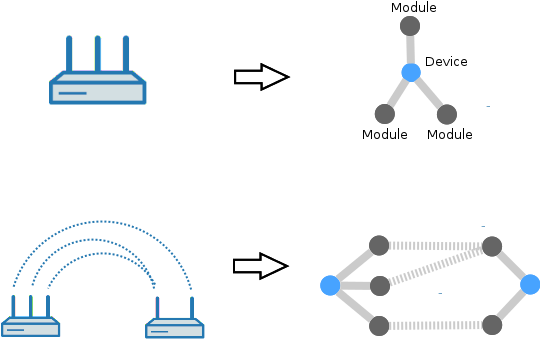
\includegraphics[width=0.5\columnwidth]{figures/apgraph.png}
      \caption{Graph representation of one (upper) and two connected accesspoints(lower)}
      \label{fig:apgraph}
    \end{figure}
    
  \subsection{Relevance of COLORING}
  \subsection{Dijkstra's Algorithm}
    TODO: How is our Channel assignment related to the problem COLORING?
    It is realated in the way that we want to assign each Module-Module-Connection a channel/color from a pool of available colors, withouth (if possible) use the same channel/color on neighboring links (meaning Aps that see each other and their traffic could lead to decreased throughput due to interference)
    Why is it not just coloring?
